\section{Improving \prgan~with richer supervision}\label{s:discussion}
This section shows how the generative models can be improved to
support higher resolution 3D shapes and by incorporating richer forms
of view-based supervision.

\subsection{Higher-resolution models}\label{s:hres}
We extend the vanilla \prgan model to handle higher resolution volumes.
There are two key modifications.
First, we replace the transposed convolutions in the generator by 
trilinear upsampling followed by a 3D convolutional layer.
In our experiments, we noticed that this modification led to smoother shapes
with less artifacts.
This fact was also verified for image generators~\cite{odena2016deconvolution}.
Second, we add a feature matching component to the generator objective.
This component acts by minimizing the difference between features computed by
the discriminator from real and fake images.
More precisely, the feature matching loss can be defined as:

\begin{equation}
	\mathcal{L}_{FM}(G, D) = \norm{\mathbb{E}_{x \sim \mathcal{D}}[D_k(x)] - 
								 \mathbb{E}_{z \sim \mathcal{N}(0, I)}[D_k(G(z))]}_2^2
\end{equation}
where $D_k(x)$ are the features from the $k$th layer of the discriminator when given
an input $x$.
In our experiments we define $k$ to be the last convolutional layer of the discriminator.
We empirically verified that this component promotes diversity in the 
generated samples and makes the training more stable.



\subsection{Using multiple cues for shape reasoning} 
So far our approach only relies on binary silhouettes for estimating
the shape, which contributes to the lack of geometric details.
One strategy is replace the projection module with a differentiable
function, \eg, a convolutional network, to approximate a sophisticated
rendering pipeline, like the one presented in~\cite{RenderNet,nalbach2016deep}. 
Such a \emph{neural renderer} could be a plug-in replacement for the
\emph{projection module} in the \prgan framework.
This would provide the ability to use collections of
realistically-shaded images for inferring probabilistic models of 3D
shapes and other properties.

We explore an alternate direction using differentiable projection
operators that do not rely on training procedures.
This choice fits well in the \prgan formulation as it does not
rely on 3D supervision for training any part of the model.
In this section, we present differentiable operators to render
depth images and semantic segmentation maps.
We demonstrate that the extra supervision enables generating more
accurate 3D shapes and allows relaxing the prior assumption
on viewpoint distribution.

\begin{figure*}[t]
\centering
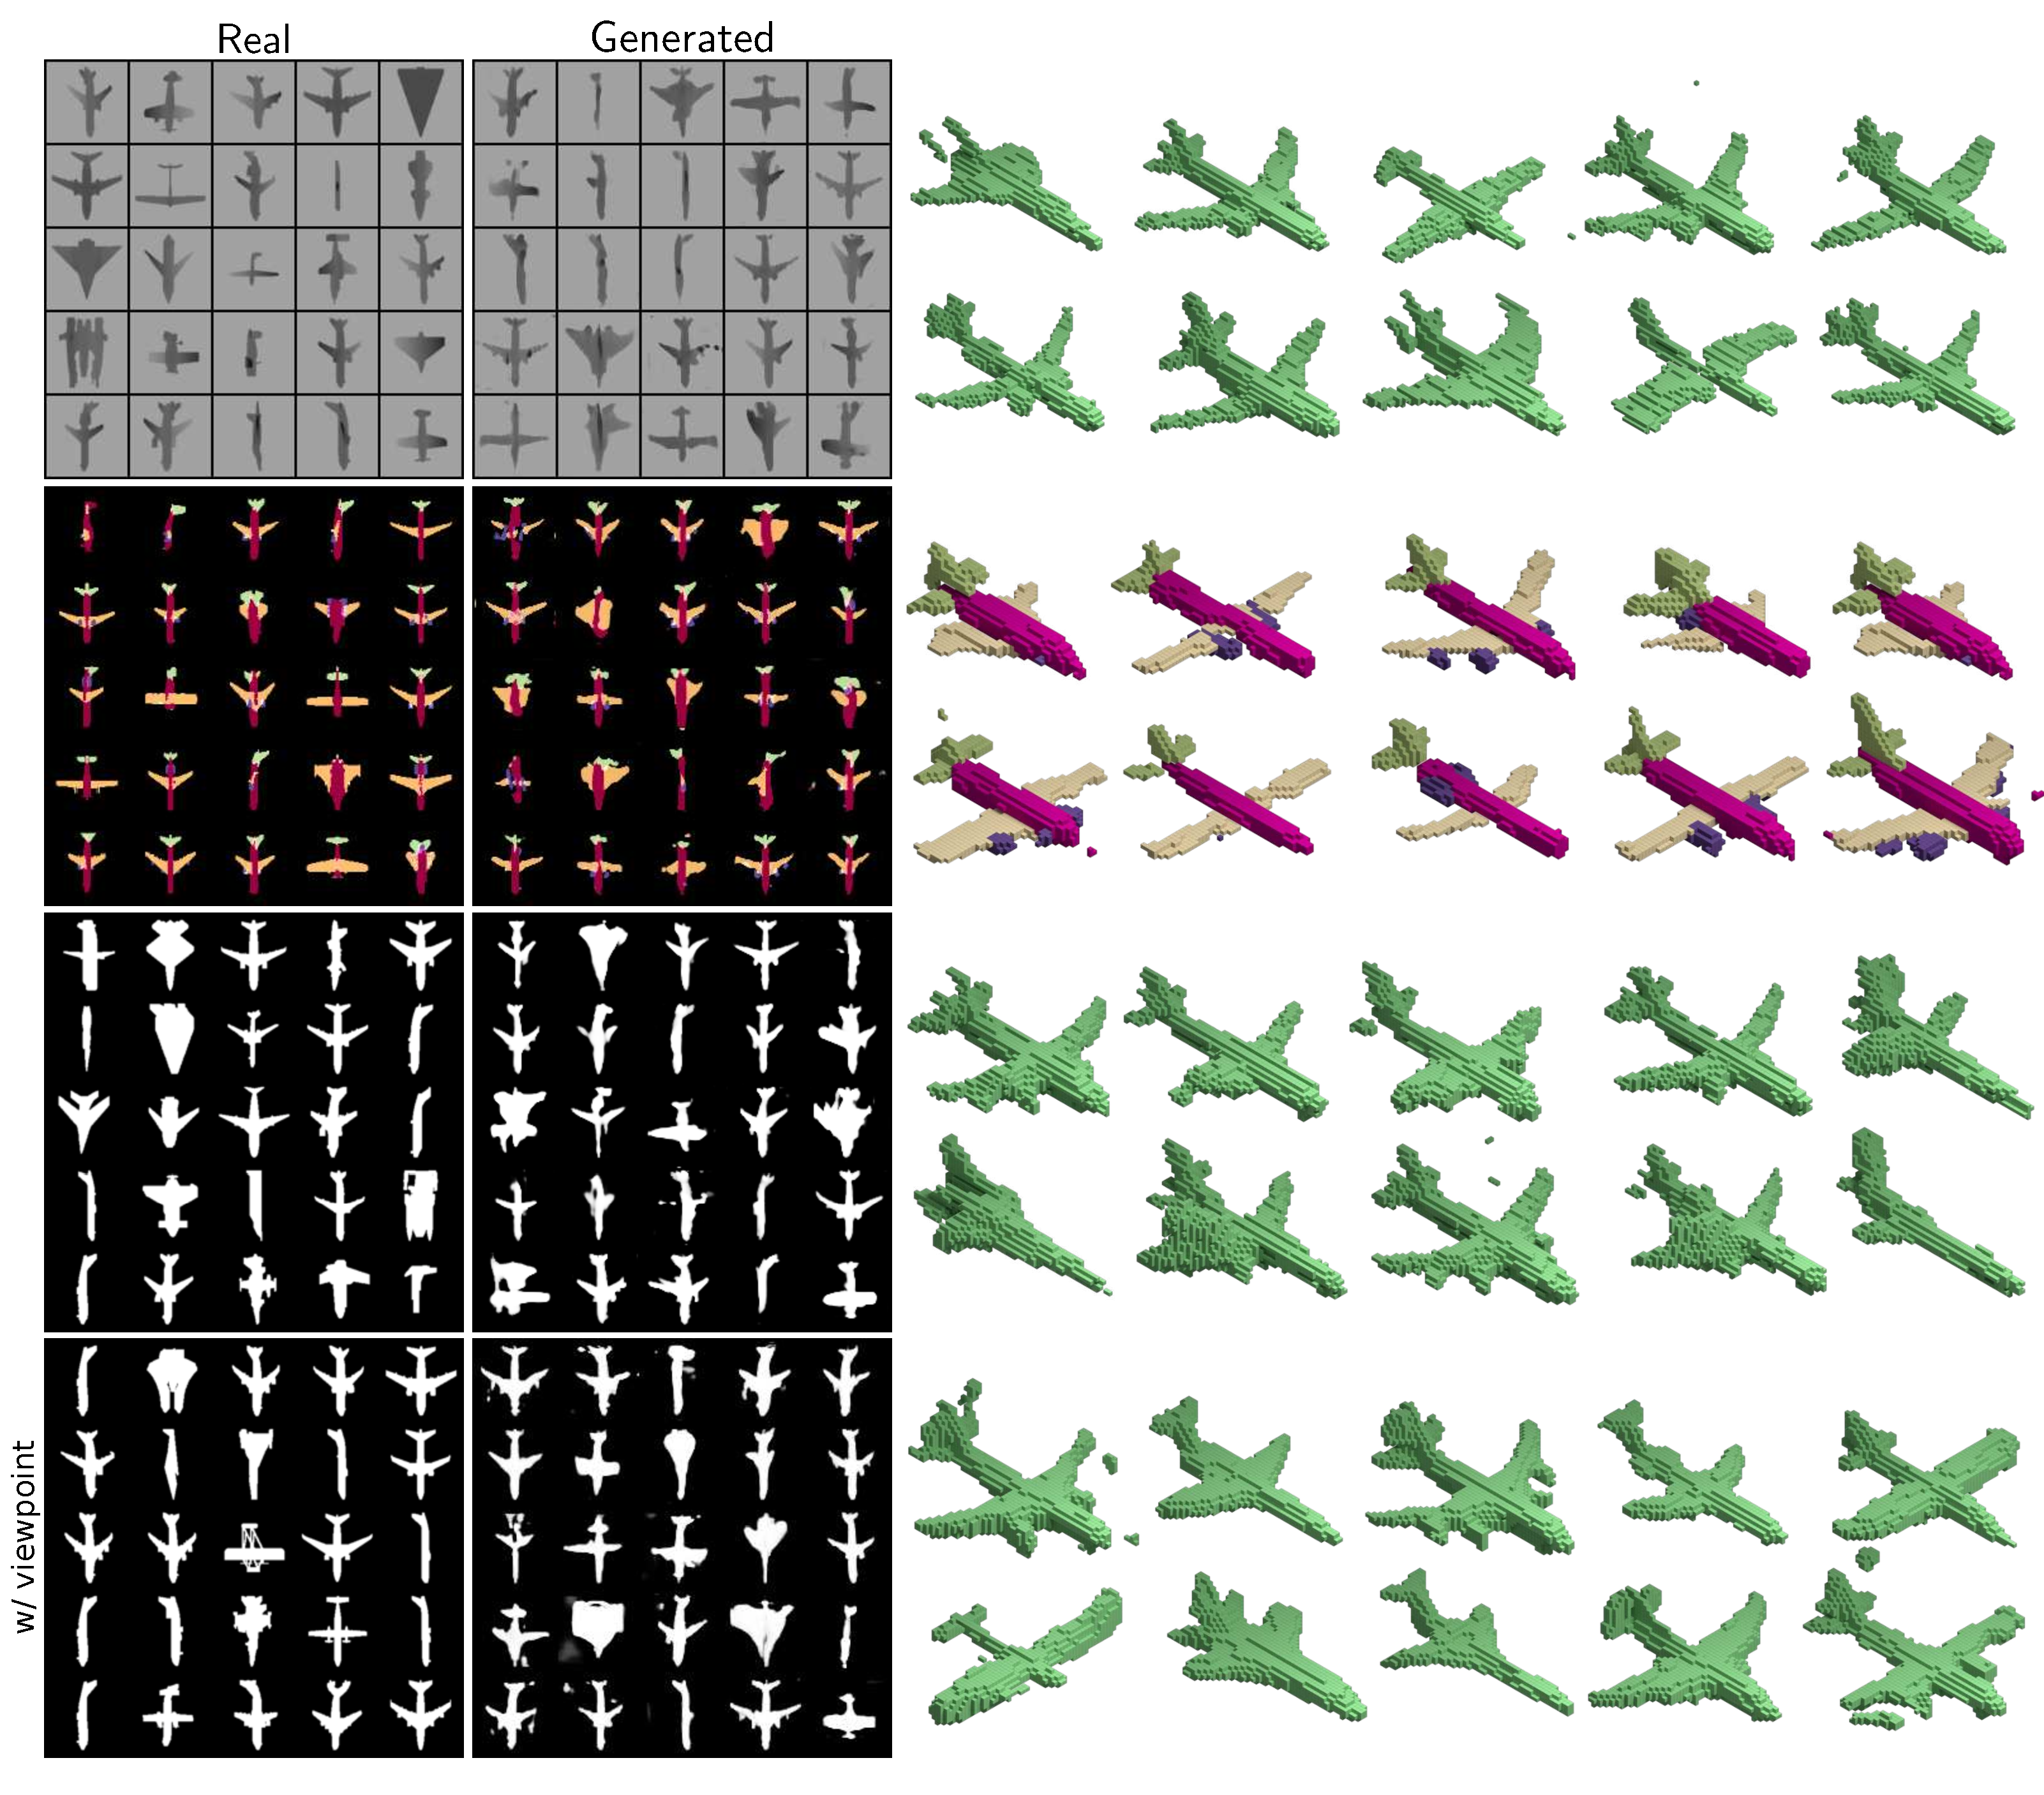
\includegraphics[width=\linewidth]{prgan/fig/new/newprojs.pdf}
\caption{\label{fig:newprojs} Shapes generated using new part segmentations and depth maps.
	From top to bottom, results using depth images, images with part segmentation, silhouettes and silhouettes annotated with viewpoints.
	Models trained with images containing additional visual cues are able to generated more accurate shapes. 
	Similarly, viewpoint annotation also helps.
	Notice that shapes generated from images with part annotation are able to generate part-annotated 3D shapes, highlighted by different colors.}
\end{figure*}

\paragraph*{Learning from depth images.}
Our framework can be adapted to learn from depth images instead of binary images.
This is done by replacing the binary projection operator $Pr$ to one that can be used to generate
depth images.
We follow an approach inspired by the binary projection.
First, we define an accessibility function $A(V, \phi, c)$ that describes whether a given voxel $c$ inside the grid $V$ is visible, 
when seen from a view $\phi$:
\begin{equation}
A(V, \phi, i, j, k) = \exp\bigg\{-\tau \sum_{l=1}^{k-1} V_\phi(i,j,l) \bigg\}.
\end{equation}

Intuitively, we are incrementally accumulating the occupancy (from the first voxel on the line of sight) as we traverse the voxel grid 
instead of summing all voxels on the entire the line of sight. 
If voxels on the path from the first to the current voxel are all
empty, the value of $A$ is 1 (indicating the current voxel is
``accessible'' to the view $\phi$). 
If there is at least one non-empty voxel on the path, the value of A
will be close to 0 (indicating this voxel is inaccessible).
A similar approach was used in our earlier work~\cite{deepshapeprior}.

Using $A$, we can define the depth value of a pixel in the projected image
as the line integral of A along the line of sight: $Pr^{D}_\phi(i,j, V)=\sum_{k}A(V,\phi,i,j,k)$. 
This operation computes the number of accessible voxels from a particular direction $\phi$, which
corresponds to the distance of the surface seen in $(i,j)$ to the camera.
Finally, we apply a smooth map to the previous operation in order to have depth values in the range $[0, 1]$.
Thus, the projection module is defined as:
\begin{equation}
\label{eq:expdepth}
	Pr^{D}_\phi((i,j),V) = 1 - \exp\bigg\{-\sum_{k}A(V,\phi,i,j,k)\bigg\}.
\end{equation}

\paragraph*{Learning from part segmentations.}
We also explore learning 3D shapes from sets of images with dense semantic annotation.
Similarly to the depth projection, we modify our projection operator to enable generation
of images whose pixels correspond to the label of particular class (or none if there is no object).
In this case, the output of the generator is multi-channel voxel grid 
$V:\mathbb{Z}^3 \times C \rightarrow [0,1] \in \mathbb{R}$, where $C$ is the number of parts present
in a particular object category.

Let $G$ to be the aggregated occupancy grid defined as $G=\sum_{c=1}^C V(i,j,k,c)$.
The semantic projection operator $Pr^{S}_\phi((i,j,c), V)$ is defined as:
\vspace{-10pt}
\begin{equation}
  Pr^{S}_\phi\left((i, j, c), V\right) = 1 - \exp\bigg\{\sum_k V_\phi(i,j,k,c) A(G_\phi, i, j, k)\bigg\},
\end{equation}
where $A$ is the accessibility operator defined previously.
Intuitively, $A(G, \phi)$ encodes if a particular voxel is visible from a viewpoint $\phi$.
When we multiply the visibility computed with the aggregated occupancy grid by the value of
a specific channel $c$ in $V$, we generate a volume that contains visibility information per part.
Finally, we take the line integral along the line of sight to generate the final image.
Examples of images and shapes generated by this operator can be seen in Figure~\ref{fig:newprojs}.

\paragraph*{Learning with viewpoint annotation.}
\label{s:viewpoint}

We also experiment with the less challenging setup where our model has access to viewpoint information
for every training image.
Notice that this problem is different from \cite{nmr,yan2016perspective}, since we still do not know
which images correspond to the same object.
Thus, multi-view losses are not a viable alternative.
Our model is able to leverage viewpoint annotation by using conditional discriminators.
The conditional discriminator has the same architecture as the vanilla discriminator but the input image is modified to contain
its corresponding viewpoint annotation.
This annotation is represented by an one-hot encoding concatenated to every pixel in the image.
For example, if a binary image from a dataset with shapes rendered from 8 viewpoints will be represented as a 9-channel image.
This procedure is done for images generated by our generator and images coming from the dataset.

\begin{table}
\centering
\setlength{\tabcolsep}{4pt}
\begin{tabular}{c|c|c|c|c}
Model  & Supervision & $\mathcal{D} \rightarrow G(z)$ & $G(z) \rightarrow \mathcal{D}$
  & Avg.  \\ 
\hline
	$\prgan^*$ & Silhouette  & 0.431   & 0.391   & 0.411 \\ 
	$\prgan^\dagger$ & Silhouette  & 0.429   & 0.391   & 0.410 \\ 
\hline
\prgan & Silhouette  & 0.442   & 0.400   & 0.421 \\ 
\prgan & Silhouette + View & 0.439  & 0.431  & 0.435 \\
\prgan & Depth & 0.497  & 0.448    & 0.472 \\
\prgan & Part Segmentation & 0.496  & 0.507  & 0.502 \\ 
\hline
3D-GAN & Volumetric & 0.538 &0.530  &0.534\\
\end{tabular}
\caption{\label{tab:newcomp} Quantitative comparison between models
  trained with different projection operators. The Chamfer similarity
  under the volumetric intersection over union (IoU) is shown for
  \prgan trained with varying amounts of supervision and a 3D-GAN
  trained with volumetric supervision. 
  The metric (higher the better) indicates that
  \prgan with richer supervision are better and approaches the
  quality of 3D-GAN. 
	$\prgan^*$ is trained using only 4 out of 8 views
	per object.
	$\prgan^\dagger$ is trained using all 8 views but for half of the
	objects.
	}
\end{table}


\subsection{Experiments}

\paragraph*{Setup.}
We generate training images using airplanes from the ShapeNet part segmentation dataset~\cite{chang2015shapenet}.
Those shapes have their surface densely annotated as belonging to one of four parts:
body, wing, tail or engine.
We render those shapes using the same viewpoint configuration described in Section~\ref{s:experiments}.
However, in this scenario we use $64\times 64$ images instead of $32\times 32$.
The models are rendered as binary silhouettes, depth maps and part segmentation masks.
We train a high resolution \prgan model for every set of rendered images using the corresponding
projection operator.
Each model is trained for 50 epochs and trained with the Adam optimizer.
We use a learning rate of $2.5 \times 10^{-3}$ for the generator and
$2 \times 10^{-5}$ for the discriminator.

\paragraph*{Evaluation.}
The models trained with different visual clues are evaluated through the following metric:
\begin{equation}
	\frac{1}{|\mathcal{D}|}\sum_{x \in \mathcal{D}} \min_{g \in \mathcal{G}} IoU(x, g) +
	\frac{1}{|\mathcal{G}|}\sum_{g \in \mathcal{G}} \min_{x \in \mathcal{D}} IoU(x, g) 
	\label{eq:metric}
\end{equation}
where $IoU$ corresponds to intersection over union, $\mathcal{G}$ is a set of generated shapes and
$\mathcal{D}$ is a set of shapes from the training data.
In our setup, both $\mathcal{G}$ and $\mathcal{D}$ contain 512 shapes.
Shapes in $\mathcal{D}$ are randomly sampled from the same dataset that originated the images,
whereas shapes in $\mathcal{G}$ are generated through $G(z)$.
Noticeably, the shapes generated by \prgan do not have the same orientation as the shapes
in $\mathcal{D}$ but are consistently oriented among themselves.
Thus, before computing Equation~\ref{eq:metric}, we select one of 8 possible transformations that minimizes
$IoU$ -- there are 8 rendering viewpoints in the training set.
Additionally, the components in Equation~\ref{eq:metric} indicate two different aspects:
the first term ($\mathcal{D}\rightarrow G(z)$) indicates how the variety in the dataset is covered whereas 
the second term ($G(z)\rightarrow \mathcal{D}$) indicates how accurate the generated shapes are.
A comparison between models trained with different projection operators can be seen in
Table~\ref{tab:newcomp}.
The model trained with part segmentation clues yields the best results.
As expected, using only silhouettes leads to worse results in both metrics and adding viewpoint
supervision improves upon this baseline.
Interestingly, depth and part segmentation supervision clues lead to models that generate shapes
with similar variety (similar $\mathcal{D}\rightarrow G(z)$).
However, shapes generated from models using part segmentation clues are more similar to the ones
in the dataset (higher $G(z)\rightarrow \mathcal{D}$).

